%\documentclass{beamer}
\documentclass[9pt,english,t,9pt]{beamer}
\beamertemplatenavigationsymbolsempty

\usepackage{amsfonts}
\usepackage{amsmath}
\usepackage{bbm}
%\usepackage{graphicx}
%\usepackage{listings}
\usepackage{epstopdf}
\usepackage{booktabs}
\usepackage{bigstrut}
\usepackage{rotating}
\usepackage{multirow}
\usepackage{threeparttable}
\usepackage{caption} % subcaption
\usepackage{hyperref}
%\usepackage{tikz}


\usepackage[utf8]{inputenc}
\usepackage[T1]{fontenc}
\usepackage{amsmath}
\usepackage{amsfonts}
\usepackage{amssymb}
\usepackage{mhchem}
\usepackage{stmaryrd}
\usepackage{graphicx}
\usepackage[export]{adjustbox}


\newenvironment{wideitemize}{\itemize\addtolength{\itemsep}{10pt}}{\enditemize}
\newenvironment{wideenumerate}{\enumerate\addtolength{\itemsep}{10pt}}{\endenumerate}


%% LyX 2.3.6.1 created this file.  For more info, see http://www.lyx.org/.
%% Do not edit unless you really know what you are doing.

\usepackage{lmodern}
\usepackage[T1]{fontenc}
\usepackage[utf8]{inputenc}
\setcounter{tocdepth}{1}
\setlength{\parskip}{\smallskipamount}
\setlength{\parindent}{0pt}
\usepackage{units}
\usepackage{amstext}
\usepackage{amssymb}
\usepackage{graphicx}
\usepackage[authoryear]{natbib}
\PassOptionsToPackage{normalem}{ulem}
\usepackage{ulem}

\makeatletter
%%%%%%%%%%%%%%%%%%%%%%%%%%%%%% Textclass specific LaTeX commands.
% this default might be overridden by plain title style
\newcommand\makebeamertitle{\frame{\maketitle}}%
% (ERT) argument for the TOC
\AtBeginDocument{%
	\let\origtableofcontents=\tableofcontents
	\def\tableofcontents{\@ifnextchar[{\origtableofcontents}{\gobbletableofcontents}}
	\def\gobbletableofcontents#1{\origtableofcontents}
}

%%%%%%%%%%%%%%%%%%%%%%%%%%%%%% User specified LaTeX commands.



\usepackage{tikz}
\usetikzlibrary{positioning}
\usepackage{appendixnumberbeamer}

\usepackage{graphicx}
\usepackage{subfig}

\usetheme[progressbar=frametitle,block=fill,subsectionpage=progressbar]{metropolis}

% margin
\setbeamersize{text margin right=1.5cm}

% colors
\colorlet{DarkRed}{red!70!black}
\setbeamercolor{normal text}{fg=black}
\setbeamercolor{alerted text}{fg=DarkRed}
\setbeamercolor{progress bar}{fg=DarkRed}
\setbeamercolor{button}{bg=DarkRed}

% width of seperators
\makeatletter
\setlength{\metropolis@titleseparator@linewidth}{1pt}
\setlength{\metropolis@progressonsectionpage@linewidth}{1pt}
\setlength{\metropolis@progressinheadfoot@linewidth}{1pt}
\makeatother

% new alert block
\newlength\origleftmargini
\setlength\origleftmargini\leftmargini
\setbeamertemplate{itemize/enumerate body begin}{\setlength{\leftmargini}{4mm}}
\let\oldalertblock\alertblock
\let\oldendalertblock\endalertblock
\def\alertblock{\begingroup \setbeamertemplate{itemize/enumerate body begin}{\setlength{\leftmargini}{\origleftmargini}} \oldalertblock}
\def\endalertblock{\oldendalertblock \endgroup}
\setbeamertemplate{mini frame}{}
\setbeamertemplate{mini frame in current section}{}
\setbeamertemplate{mini frame in current subsection}{}
\setbeamercolor{section in head/foot}{fg=normal text.bg, bg=structure.fg}
\setbeamercolor{subsection in head/foot}{fg=normal text.bg, bg=structure.fg}

% footer
\makeatletter
\setbeamertemplate{footline}{%
	\begin{beamercolorbox}[colsep=1.5pt]{upper separation line head}
	\end{beamercolorbox}
	\begin{beamercolorbox}{section in head/foot}
		\vskip1pt\insertsectionnavigationhorizontal{\paperwidth}{}{\hskip0pt plus1filll \insertframenumber{} / \inserttotalframenumber \hskip2pt}\vskip3pt% 
	\end{beamercolorbox}%
	\begin{beamercolorbox}[colsep=1.5pt]{lower separation line head}
	\end{beamercolorbox}
}
\makeatother

% toc
\setbeamertemplate{section in toc}{\hspace*{1em}\inserttocsectionnumber.~\inserttocsection\par}
\setbeamertemplate{subsection in toc}{\hspace*{2em}\inserttocsectionnumber.\inserttocsubsectionnumber.~\inserttocsubsection\par}


% Automatically create vspace between items
% See: https://tex.stackexchange.com/questions/369504/beamer-vertically-stretching-level-1-list-items-in-a-nested-list-environment
%\usepackage{xpatch} 
%\xpatchcmd{\itemize}   
%	{\def\makelabel}   
%	{\ifnum\@itemdepth=1\relax      
%		\setlength\itemsep{\fill} % separation for first level    
%		\fi\def\makelabel   
%	}{}{} 
%\xpatchcmd{\enditemize}   
%	{\endlist}   
%	{\endlist\ifnum\@itemdepth<2\else\vfil\fi}{}{}




%% Automatically create vspace between items
%% See: https://jayrobwilliams.com/posts/2019/10/better-beamer
%\makeatletter
%\renewcommand{\itemize}[1][]{%
%	\beamer@ifempty{#1}{}{\def\beamer@defaultospec{#1}}%
%	\ifnum \@itemdepth >2\relax\@toodeep\else
%	\advance\@itemdepth\@ne
%	\beamer@computepref\@itemdepth% sets \beameritemnestingprefix
%	\usebeamerfont{itemize/enumerate \beameritemnestingprefix body}%
%	\usebeamercolor[fg]{itemize/enumerate \beameritemnestingprefix body}%
%	\usebeamertemplate{itemize/enumerate \beameritemnestingprefix body begin}%
%	\list
%	{\usebeamertemplate{itemize \beameritemnestingprefix item}}
%	{\def\makelabel##1{%
%			{%
%				\hss\llap{{%
%						\usebeamerfont*{itemize \beameritemnestingprefix item}%
%						\usebeamercolor[fg]{itemize \beameritemnestingprefix item}##1}}%
%			}%
%		}%
%	}
%	\fi%
%	\setlength\itemsep{\fill}
%	\ifnum \@itemdepth >1
%	\vfill
%	\fi%  
%	\beamer@cramped%
%	\raggedright%
%	\beamer@firstlineitemizeunskip%
%}
%
%\def\enditemize{\ifhmode\unskip\fi\endlist%
%	\usebeamertemplate{itemize/enumerate \beameritemnestingprefix body end}
%	\ifnum \@itemdepth >1
%	\vfil
%	\fi%  
%}
%\makeatother
%
%\makeatother



% Broer et al
\usepackage[T1]{fontenc}
\usepackage{graphicx, amsmath, tabularx}
\usetheme{default}
\usepackage{tikz}
\newcommand\RBox[1]{%
	\tikz\node[draw,rounded corners,align=center,] {#1};%
}  
%\setbeamercovered{transparent}
\usepackage{soul}
\usepackage{natbib}
\usepackage[makeroom]{cancel}
\bibliographystyle{econometrica}

\newcommand{\ben}{\begin{enumerate}}
	\newcommand{\een}{\end{enumerate}}

\newcommand{\bit}{\begin{itemize}}
	\newcommand{\eit}{\end{itemize}}

\newcommand{\lb}{\label}
\newcommand{\re}{\eqref}




\DeclareUnicodeCharacter{00A0}{ }


\usepackage{babel}
\begin{document}
	\title{12. Analytical HANK \vspace{-2mm}}
	\subtitle{Adv. Macro: Heterogenous Agent Models} 
	\author{Jeppe Druedahl \& Patrick Moran}
	\date{2022}
	
	{
		\setbeamertemplate{footline}{} 
		\begin{frame}
		
		\maketitle
		
		\begin{tikzpicture}[overlay, remember picture]
		\node[above left=0cm and 0.0cm of current page.south east] 
		{
\includegraphics[width=4cm]{../05/figs/KUSAMFtitlelrcorner.pdf}};
		\end{tikzpicture}
		
		\begin{tikzpicture}[overlay, remember picture]
		\node[below left=0.5cm and .8cm of current page.north east] 
		{\includegraphics[width=1.5cm]{../05/figs/KUSAMFlogo.pdf}};
		\end{tikzpicture}
		
		\begin{tikzpicture}[overlay, remember picture]
		\node[below right=0.5cm and 0.8cm of current page.north west] 
		{
\includegraphics[width=1.5cm]{../05/figs/CEBI.png}};
		\end{tikzpicture}
		
		\begin{tikzpicture}[overlay, remember picture]
		\node[above right=0.5cm and 0.8cm of current page.south west] 
		{
\includegraphics[width=1.5cm]{../05/figs/DNRF.png}};
		\end{tikzpicture}
		
	\end{frame}
}

\addtocounter{framenumber}{-1}


\section{Introduction}
\begin{frame}{Disclaimer}
\vspace{-2mm}

\vspace{20mm}
\begin{itemize}
	\item Note: The views expressed in this presentation are those of the author
	and do not represent the views of the Federal Reserve Board or Federal
	Reserve System.
\end{itemize}
\end{frame}
%
\begin{frame}{Analytical HANK}
\vspace{-2mm}
\begin{itemize}
	
\item <+->\textbf{Previously:} Learned to solve and simulate quantitative HANK models with rich household heterogeneity \vfill

\item <+->\textbf{Challenge:} In large models with many moving parts, often difficult to understand the main mechanisms driving the results \vfill 

\item <+->\textbf{Goal for today:} Derive analytical solutions to simplified HANK models to better understand the main transmission mechanisms \vfill

\item <+->\textbf{Central economic questions:}
\begin{enumerate}
	\item What are the main mechanisms driving monetary policy transmission in standard HANK and RANK models? 
	\item Does it matter whether we include price rigidities or wage rigidities in the model?
	\item Is the fiscal multiplier greater than or less than one? What mechanisms drive this?
\end{enumerate}
\end{itemize}
\end{frame}



\begin{frame}{Analytical HANK}
\vspace{-2mm}
\begin{itemize}
	
\item <+->\textbf{Today:} To answer these questions, helpful to look at solutions coming from simplified models solved with paper and pencil \vfill\vfill

\item <+->\textbf{Key insight:} Possible to turn off liquidity in simple HANK models, so that there is no risk sharing (in contrast: RANK models have full risk sharing, quantitative HANK models have partial risk sharing) \vfill\vfill

\item <+->\textbf{Plan for today:}
\begin{enumerate}
	\item Learn to solve the zero-liquidity analytical HANK model\vfill
	\item Study monetary transmission, the role of firm profits, and the distinction between price and wage rigidities\vfill
	\item Study fiscal policy and the role of intertemporal MPCs
\end{enumerate}
\end{itemize}
\end{frame}
%



\section{Zero Liquidity HANK Model}


\begin{frame}{Model framework}
\bit
\setlength\itemsep{1.5em}	

\item We'll begin with a simple HANK model following Broer et al (2020)
\pause


\item We'll include two types of households: workers ands capitalists
\bit
\item Ex ante identical except that capitalists own the firms 
\eit
\pause

\item Workers face idiosyncratic productivity risk
\bit
\item Workers ex ante identical, ex post different because of different realizations of productivity shocks
\eit
\pause

\item All households can trade in riskless bond subject to a ``very tight'' borrowing constraint

\eit
\end{frame}


\begin{frame}{Simple HANK model}

\bit
\setlength\itemsep{1.5em}


\item Household side: workers and capitalists
\bit
\item Capitalists collects firm dividends, workers do not
\item Idiosyncratic productivity risk
\item Participation cost of working 
\item Choose how much to work, consume and save 
\item In equilibrium: capitalists choose not to work
\eit

\pause


\item Firm side: closely follows Gal\'{i} (2009)
\bit
\item Monopolistic firms
\item Use labor inputs
\item Set prices subject to the Calvo friction
\eit 

%\item Structure close to Ravn-Sterk (2017)
\pause

\item Motivation: Tractable form of type-heterogeneity that matches
\ben 
\item A small share of the households own almost all financial wealth (Piketty-Zucman, 2015)
\item At the top of the wealth distribution, labor income is a small share of total income (Gornemann-Kuester-Nakajima, 2016)
\een

\pause
\item Later: compare the solution to a textbook RANK model
\eit

\end{frame}





\begin{frame}{HANK model: Households}

\bit
\setlength\itemsep{0.5em}
\item<+-> Worker $j \in [0,1]$ solves:
\begin{eqnarray}
\max_{C_{jt}, N_{jt}, B_{jt}} &&  E_t \sum_{k=0}^{\infty} \beta^k \left(\log(C_{jt}) - \frac{N_{jt}^{1+\varphi}}{1+\varphi}{\color{red} - \vartheta *\mathbb{I}_{N_{jt}>0}}\right) \nonumber  \\
\text{s.t.}&&P_{t} C_{jt} + Q_{t} B_{jt} \leq {\color{red}W_{jt}} N_{jt} + B_{jt-1} \nonumber \\
&& {\color{red}B_{jt}\geq 0} \label{no_borrowing} \nonumber
\end{eqnarray}

\item<+-> Capitalist $j \in (1,m_c]$ solves:
\begin{eqnarray}
\max_{C_{jt}, N_{jt}, B_{jt}} &&  E_t \sum_{k=0}^{\infty} \beta^k \left(\log(C_{jt}) - \frac{N_{jt}^{1+\varphi}}{1+\varphi}{\color{red} - \vartheta *\mathbb{I}_{N_{jt}>0}}\right) \nonumber  \\
\lb{capitalist_bc}
\text{s.t.}&&P_{t} C_{jt} + Q_{t} B_{jt} \leq {\color{red}W_{jt}} N_{jt} + B_{jt-1} + {\color{red} P_t D_{jt}} \nonumber \\
&& {\color{red}B_{jt}\geq 0} \label{no_borrowing} \nonumber
\end{eqnarray}
\item<+-> Assumption 1: capitalists split the well-diversified portfolio of firm claims equally, $\rightarrow$ $D_{jt} = \frac{D_t}{m_c}$
\item<+-> Assumption 2: $m_c$ small $\rightarrow$ capitalists choose not to work 
\eit

\end{frame}


\begin{frame}{HANK model: Production side}

\bit
\setlength\itemsep{2em}
\item CES demand for intermediate goods :
\begin{eqnarray}
Y_{it} = \left(\frac{P_{it}}{P_t}\right)^{-\epsilon}Y_t \nonumber
\end{eqnarray} 

\pause
\item Intermediate goods producer $i$ uses production technology
\begin{eqnarray}
Y_{it}  = \int_{j=0}^{1} A_{jt} N_{jit} dj \nonumber
\end{eqnarray}

\pause
\item where $A_{jt}$ is the productivity of household $j$, $A_{j} \sim F$ with finite support and $E(A_{j})=1$

\pause
\item Calvo friction and intermediate firm maximization problem otherwise identical
\eit

\end{frame}

\begin{frame}{HANK model}

\bit
\item Government
\bit
\setlength\itemsep{2em}
\item Fiscal authority does nothing -- no taxation nor government debt
\item Central bank follows Taylor rule:
\begin{eqnarray}
\lb{nonlogtaylor}
&& \frac{1}{Q_t} = \frac{1}{\beta}\Pi_t^{\phi_{\pi}}e^{\nu_t} \nonumber \\
\Rightarrow && \hat i_t = \phi_{\pi}\pi^p_t + \nu_t \nonumber
\end{eqnarray}
\eit

\pause 

\item Equilibrium conditions:
\begin{eqnarray}
\lb{goods_clearing}
\int_{j=0}^{1+m_c} C_{jt} dj &=& Y_{t}  \nonumber\\
\lb{bonds_clearing}
\int_{0}^{1+m_c} B_{jt} dj  &=& 0 \nonumber
\end{eqnarray}
\eit
\end{frame}

\begin{frame}{Solution of the simple HANK model}

\bit
\setlength\itemsep{2em}


\item Most HANK models do not admit an analytical solution
\bit
\item Why? The wealth distribution is an endogenous state variable 
\eit
\pause

\item In contrast, this simple HANK model is possible to solve
\bit
\item Zero borrowing constraint $\rightarrow$ Degenerate equilibrium bond wealth distribution 
\bit
\item Also used in Krusell-Mukoyama-Smith (2011), Werning (2015); McKay-Reis (2016); Ravn-Sterk (2016)
\item ``Autarky solution'' $\rightarrow$ Workers consume labor income hand-to-mouth 
\item Similarly, capitalists consume profit income hand-to-mouth
\eit	

\pause	
\item Individual worker consumption is linear in aggregate worker consumption

\item Individual capitalist consumption is linear in agg. capitalist consumption

\item Reduced form representation: two-agent model
%\bit
%\item TANK models also analyzed in Debortoli-Gali (2017) and Bilbiie (2017)
%\eit
\eit

\pause
\item Next: Derivation of the equilibrium in our simple HANK model
\eit

\end{frame}

\begin{frame}{Aggregation I - Labour supply}

\bit
\setlength\itemsep{2em}
\item No borrowing + zero net supply of assets $\rightarrow$ The equilibrium must coincide with autarky
\pause

\item Worker consumption:
\begin{eqnarray}
\lb{cond1}
C_{jt} = \frac{W_{jt}}{P_{t}} N_{jt}
\end{eqnarray}

\pause
\item Intratemporal first order condition:
\begin{eqnarray}
\lb{cond2}
\frac{W_{jt}}{P_t} = MRS_{jt} = N_{jt}^{\varphi}C_{jt}
\end{eqnarray}

\pause
\item \eqref{cond1} + \eqref{cond2} $\Rightarrow$ $N_{it} = N_{jt} \hspace{3mm} \forall i,j \in [0,1]$

\pause
\item \bf Workers all supply the same amount of labour \normalfont

\eit

\end{frame}


\begin{frame}{Aggregation II - Consumption}

\bit
\setlength\itemsep{1em}

\item <+-> Define the aggregate per efficiency unit wage and aggregate supply of labor efficiency units:
\begin{eqnarray}
W_t = \int_{j=0}^{1} \frac{W_{jt}}{A_{jt}} dj \hspace{10mm} N_t  = \int_{j=0}^{1} A_{jt} N_{jt} dj \nonumber
\end{eqnarray}

\item <+-> Because labor inputs are perfectly substitutable:
\begin{eqnarray}
\lb{comp_labor_market}
W_t &=& \frac{W_{jt}}{A_{jt}} \hspace{5mm} \forall j. \nonumber
\end{eqnarray}

\item <+-> Because workers all supply the same amount of labour:
\begin{eqnarray}
\lb{comp_labor_market}
N_t &=& N_{jt} \hspace{5mm} \forall j. \nonumber
\end{eqnarray}

\item <+-> \bf Worker $j$ consumption is proportional to aggregate worker consumption: \normalfont
\begin{eqnarray}
\lb{aggregation}
C_{jt} = \frac{W_{jt}}{P_t} N_{jt} =  A_{jt} \frac{W_{jt}}{A_{jt} P_t} N_{jt} =  A_{jt} \frac{W_t}{P_t} N_{t} = A_{jt} C_t \nonumber  
\end{eqnarray}
where $C_t \equiv \frac{W_t}{P_t} N_t$
\eit

\end{frame}

\begin{frame}{Aggregate Euler equation}

\bit
\setlength\itemsep{1.5em}

\item $Q_t$ must adapt so that no household chooses to save in equilibrium.
\pause
\item Household $j$ intertemporal optimality condition:
\begin{eqnarray}
Q_{t} &=& \beta E_{t} \left\{ \left(\frac{C_{jt+1}}{C_{jt}}\right)^{-1} \frac{P_{t}}{P_{t+1}} +\upsilon_{jt} \right\}. \nonumber
\end{eqnarray}
\pause
\item The household with the lowest consumption growth, ``the marginal saver'', must be indifferent between saving and borrowing with $\upsilon_{jt} = 0$
\pause
\item All other households are constrained with $\upsilon_{jt}>0$.
\pause
\item Who is the marginal saver?

\eit

\end{frame}

\begin{frame}{Aggregate Euler equation cont.}

\bit
\setlength\itemsep{0.45em}
\item Capitalist expected consumption growth: $E_t \frac{D_{t+1}}{D_t}$
\pause 

\item Worker expected consumption growth: $E_t \frac{A_{jt+1}C_{t+1}}{A_{jt}C_t}$
\pause 

\item Assume aggregate shocks are small in relation to idiosyncratic shocks 
\pause 
\bit
\item[] $\rightarrow$ \bf the "marginal saver" is the worker with lowest expected productivity growth: \normalfont
\begin{eqnarray}
\lb{aggregate_euler}
Q_{t} &=& \beta^{eff} E_{t} \left\{\frac{C^{-1}_{t+1}}{C^{-1}_{t}} \frac{P_{t}}{P_{t+1}}\right\} \nonumber \\
\beta^{eff} &=& \beta \max \Bigg\{E_t \left[ \left(\frac{A_{jt+1}}{A_{jt}}\right)^{-1}\right] \Bigg\}>\beta \nonumber
\end{eqnarray}
\pause 
\eit 

\item Note: steady state interest rate smaller but elasticity of aggregate consumption to interest rate is \emph{as if} in RANK (Werning, 2015)
\pause 

\item Log-linearize Euler equation and aggregation result around steady state:
\begin{eqnarray}
\hat c_t &=& E_t \hat c_{t+1} - (\hat i_t - E_t \pi_{t+1}) \nonumber \\
\hat c_t &=& \hat \omega_t + \hat n_t \nonumber
\end{eqnarray}
\eit

\end{frame}







\begin{frame}{Other equilibrium conditions}

\bit
\setlength\itemsep{1.5em}
\item On firm side, log-linearization of first order condition implies the standard Phillips curve:
\begin{eqnarray}
\pi^p_t = \beta E_t \pi^p_{t+1}+\lambda_p \hat{mc}_t \nonumber
\end{eqnarray}
\bit
\item where $\lambda_p \equiv \frac{(1-\theta_p)(1-\beta \theta_p)}{\theta_p}$
\item with CRS production technology, $\hat{mc}_t = \hat \omega_t$
\eit
\pause
\item Intratemporal optimality condition:
\begin{eqnarray}
&& \frac{W_{jt}}{P_t}=C_{jt}N_{jt}^{\varphi}  \nonumber \\
\Leftrightarrow && \frac{W_{t}}{P_t}=A_{jt}C_tN_t^{\varphi}  \nonumber \\
\Rightarrow && \hat \omega_{t} = \varphi \hat n_{t} + \hat c_{t} \nonumber
\end{eqnarray}
\eit

\end{frame}



\begin{frame}{Summary of log-linearized equilibrium}

\bit
\item Our simple HANK model:
\begin{eqnarray}
\lb{Phillips_final}
\text{Phillips}: && \pi^p_t = \beta E_t \pi^p_{t+1}+\lambda_p \hat{\omega}_t \nonumber\\
\lb{IS_final}
\text{IS}: && \hat c_t = E_t \hat c_{t+1} - (\hat i_t - E_t \pi_{t+1}) \nonumber\\
\lb{Taylor_final}
\text{Taylor rule}: && \hat i_t = \phi_{\pi}\pi^p_t + \nu_t \nonumber\\
\lb{LS_final}
\text{Labor supply}: && \hat \omega_{t} = \varphi \hat n_{t} + \hat c_{t} \nonumber\\
\lb{MC_final}
\text{Market clearing}: && \hat c_{t} = \hat \omega_t  + \hat n_{t} \nonumber
\end{eqnarray}
\pause 
\item Next step: how does this compare with a textbook RANK model?
\eit

%\bit
%\item Textbook model:
%\begin{eqnarray}
%\lb{rep_Phillips_final}
%\text{Phillips}: && \pi^p_t = \beta E_t \pi^p_{t+1}+\lambda_p \hat{\omega}_t \nonumber\\
%\lb{rep_IS_final}
%\text{IS}: && \hat c_t = E_t \hat c_{t+1} - (\hat i_t - E_t \pi_{t+1}) \nonumber\\
%\lb{rep_Taylor_final}
%\text{Taylor rule}: && \hat i_t = \phi_{\pi}\pi^p_t + \nu_t \nonumber\\
%\lb{rep_LS_final}
%\text{Labor supply}: && \hat \omega_{t} = \varphi \hat n_{t} + \hat c_{t} \nonumber\\
%\lb{rep_MC_final}
%\text{Market clearing}: && \hat c_{t} = \bar{S}(\hat \omega_t  + \hat n_{t})+(1-\bar{S})\hat d_t \nonumber
%\end{eqnarray}
%where $\bar{S} = \frac{W_t N_t}{Y_t P_t} = \frac{\epsilon_p-1}{\epsilon_p}$ is the steady state labor share
%\eit

\end{frame}

\subsection{Comparison with RANK Model}

\begin{frame}{Textbook RANK model}
\bit
\setlength\itemsep{1.5em}
\item Departure point: Gal\'{i} (2009), Ch. 3

\item Household side: representative agent
\bit
\item collects labor and profit income 
\item chooses how much to work, consume and save each period
\eit
\item Firm side: Monopolistic firms
\bit
\item use labor inputs
\item set prices subject to the Calvo friction
\eit

\eit 
\end{frame}





\begin{frame}{Textbook model: Households}

\bit
\item The representative agent solves:
\begin{eqnarray}
\max_{C_{t}, B_{t}, N_t} && E_0 \sum_{t=0}^{\infty} \beta^t \left( \log (C_{t})-\frac{N_t^{1+\varphi}}{1+\varphi}\right) \nonumber \\
\text{s.t.} && P_t C_{t} + Q_{t} B_{t} \leq B_{t-1} + W_t N_t + P_t D_t \nonumber 
\end{eqnarray}

\eit

\end{frame}




\begin{frame}{Textbook model: Production side}

\bit
\setlength\itemsep{1em}
\item A competitive final goods producer assembles intermediate goods using the Dixit-Stiglitz aggregator $\rightarrow$ CES demand for intermediate goods: 
\begin{eqnarray}
Y_{it} = \left(\frac{P_{it}}{P_t}\right)^{-\epsilon}Y_t \nonumber
\end{eqnarray} 
\pause\item Intermediate goods producer $i$ uses production technology
\begin{eqnarray}
Y_{it} = N_{it}\nonumber
\end{eqnarray}
\pause\item Calvo fricition: Intermediate goods firms can only reset prices with probability $1-\theta$

\pause\item A resetting firm maximizes the sum of expected discounted profits subject to the demand function
\eit

\end{frame}



\begin{frame}{Textbook model: other conditions}

\bit

\setlength\itemsep{2em}
\item Fiscal authority does nothing -- no taxation nor government debt\pause
\item Central bank follows Taylor rule:
\begin{eqnarray}
\lb{nonlogtaylor}
&& \frac{1}{Q_t} = \frac{1}{\beta}\Pi_t^{\phi_{\pi}}e^{\nu_t} \nonumber \\
\Rightarrow && \hat i_t = \phi_{\pi}\pi^p_t + \nu_t \nonumber
\end{eqnarray}
\pause

\item Equilibrium conditions:
\begin{eqnarray}
\lb{goods_clearing}
C_{t} &=& Y_{t} \nonumber \\
B_{t} &=& 0 \hspace{5mm} \nonumber
\end{eqnarray}

\pause
\item Textbook RANK model is easy to solve
\bit
\item Up to the first order, the state space consist only of aggregate variables
\item (Fluctuations in price dispersion are second order)
\eit
\eit



\end{frame}


% ==========================================



\begin{frame}{Summary of log-linearized equilibrium}

\bit
\item Textbook RANK model:
\begin{eqnarray}
\lb{rep_Phillips_final}
\text{Phillips}: && \pi^p_t = \beta E_t \pi^p_{t+1}+\lambda_p \hat{\omega}_t \nonumber\\
\lb{rep_IS_final}
\text{IS}: && \hat c_t = E_t \hat c_{t+1} - (\hat i_t - E_t \pi_{t+1}) \nonumber\\
\lb{rep_Taylor_final}
\text{Taylor rule}: && \hat i_t = \phi_{\pi}\pi^p_t + \nu_t \nonumber\\
\lb{rep_LS_final}
\text{Labor supply}: && \hat \omega_{t} = \varphi \hat n_{t} + \hat c_{t} \nonumber\\
\lb{rep_MC_final}
\text{Market clearing}: && \hat c_{t} = \bar{S}(\hat \omega_t  + \hat n_{t})+(1-\bar{S})\hat d_t \nonumber
\end{eqnarray}
where $\bar{S} = \frac{W_t N_t}{Y_t P_t} = \frac{\epsilon_p-1}{\epsilon_p}$ is the steady state labor share
\eit

\invisible{
\bit
\item Our simple HANK model:
\begin{eqnarray}
\lb{Phillips_final}
\text{Phillips}: && \pi^p_t = \beta E_t \pi^p_{t+1}+\lambda_p \hat{\omega}_t \nonumber\\
\lb{IS_final}
\text{IS}: && \hat c_t = E_t \hat c_{t+1} - (\hat i_t - E_t \pi_{t+1}) \nonumber\\
\lb{Taylor_final}
\text{Taylor rule}: && \hat i_t = \phi_{\pi}\pi^p_t + \nu_t \nonumber\\
\lb{LS_final}
\text{Labor supply}: && \hat \omega_{t} = \varphi \hat n_{t} + \hat c_{t} \nonumber\\
\lb{MC_final}
\text{Market clearing}: && {\color{red}\hat c_{t} = \hat \omega_t  + \hat n_{t}} \nonumber
\end{eqnarray}
\eit
}

\end{frame}


\begin{frame}{Summary of log-linearized equilibrium}

\bit
\item Textbook RANK model:
\begin{eqnarray}
\lb{rep_Phillips_final}
\text{Phillips}: && \pi^p_t = \beta E_t \pi^p_{t+1}+\lambda_p \hat{\omega}_t \nonumber\\
\lb{rep_IS_final}
\text{IS}: && \hat c_t = E_t \hat c_{t+1} - (\hat i_t - E_t \pi_{t+1}) \nonumber\\
\lb{rep_Taylor_final}
\text{Taylor rule}: && \hat i_t = \phi_{\pi}\pi^p_t + \nu_t \nonumber\\
\lb{rep_LS_final}
\text{Labor supply}: && \hat \omega_{t} = \varphi \hat n_{t} + \hat c_{t} \nonumber\\
\lb{rep_MC_final}
\text{Market clearing}: && {\color{red}\hat c_{t} = \bar{S}(\hat \omega_t  + \hat n_{t})+(1-\bar{S})\hat d_t} \nonumber
\end{eqnarray}
%where $\bar{S} = \frac{W_t N_t}{Y_t P_t} = \frac{\epsilon_p-1}{\epsilon_p}$ is the steady state labor share
\eit

\bit
\item Our simple HANK model:
\begin{eqnarray}
\lb{Phillips_final}
\text{Phillips}: && \pi^p_t = \beta E_t \pi^p_{t+1}+\lambda_p \hat{\omega}_t \nonumber\\
\lb{IS_final}
\text{IS}: && \hat c_t = E_t \hat c_{t+1} - (\hat i_t - E_t \pi_{t+1}) \nonumber\\
\lb{Taylor_final}
\text{Taylor rule}: && \hat i_t = \phi_{\pi}\pi^p_t + \nu_t \nonumber\\
\lb{LS_final}
\text{Labor supply}: && \hat \omega_{t} = \varphi \hat n_{t} + \hat c_{t} \nonumber\\
\lb{MC_final}
\text{Market clearing}: && {\color{red}\hat c_{t} = \hat \omega_t  + \hat n_{t}} \nonumber
\end{eqnarray}
where $\hat c_{t}$ is now the deviation in the aggregate consumption of workers
\eit



\end{frame}



\begin{frame}{HANK vs RANK}

\bit
\setlength\itemsep{1em}
\item Key difference: which consumption aggregate enters into the IS curve 
\pause
\item Textbook RANK model: the consumption aggregate depends on both labor income and firm profits
$$ \hat c_{t} = \bar{S}(\hat \omega_t  + \hat n_{t})+(1-\bar{S})\hat d_t $$
\pause
\item Simple HANK model: the consumption aggregate in the IS curve depends only on labor income (firm profits irrelevant)
$$ \hat c_{t} = \hat \omega_t  + \hat n_{t} $$
\pause
\item Should we be concerned about the fact that firm profits are so important in the RANK model? Most households do not own firms...
\eit

\end{frame}



% -------------------------------------------------------------

\section{Monetary Policy Transmission}
%\subsection{The Role of Firm Profits}


\begin{frame}{Our goal}

\bf Inspect the monetary transmission mechanism in simple HANK model \normalfont
\bit
\setlength\itemsep{0.5em}
\item Tractable model that admits analytical solutions

\item Compare response to monetary shock to textbook RANK model 

\item Compare under two forms of nominal rigidities: rigid prices and rigid wages
\eit
\end{frame}


\begin{frame}{A monetary experiment}
\bit
\setlength\itemsep{1.5em}
\item Let's feed in a shock to the Taylor Rule:
\begin{eqnarray}
\hat i_t = \phi_{\pi}\pi^p_t + \nu_t \nonumber
\end{eqnarray}
\item Assume AR(1): $\nu_t = \rho_{\nu} \nu_{t-1}+\epsilon_{\nu t}$
\item Feed in a 25 basis point shock with $\rho_{\nu}=0.5$
\item How do the two models respond?
\item Other parameters follow Gal\'{i} (2008)
\eit
\end{frame}


\begin{frame}[t]{Monetary Shock: Consumption, Output and Inflation}
\begin{figure}[h]  
\begin{flushleft}
	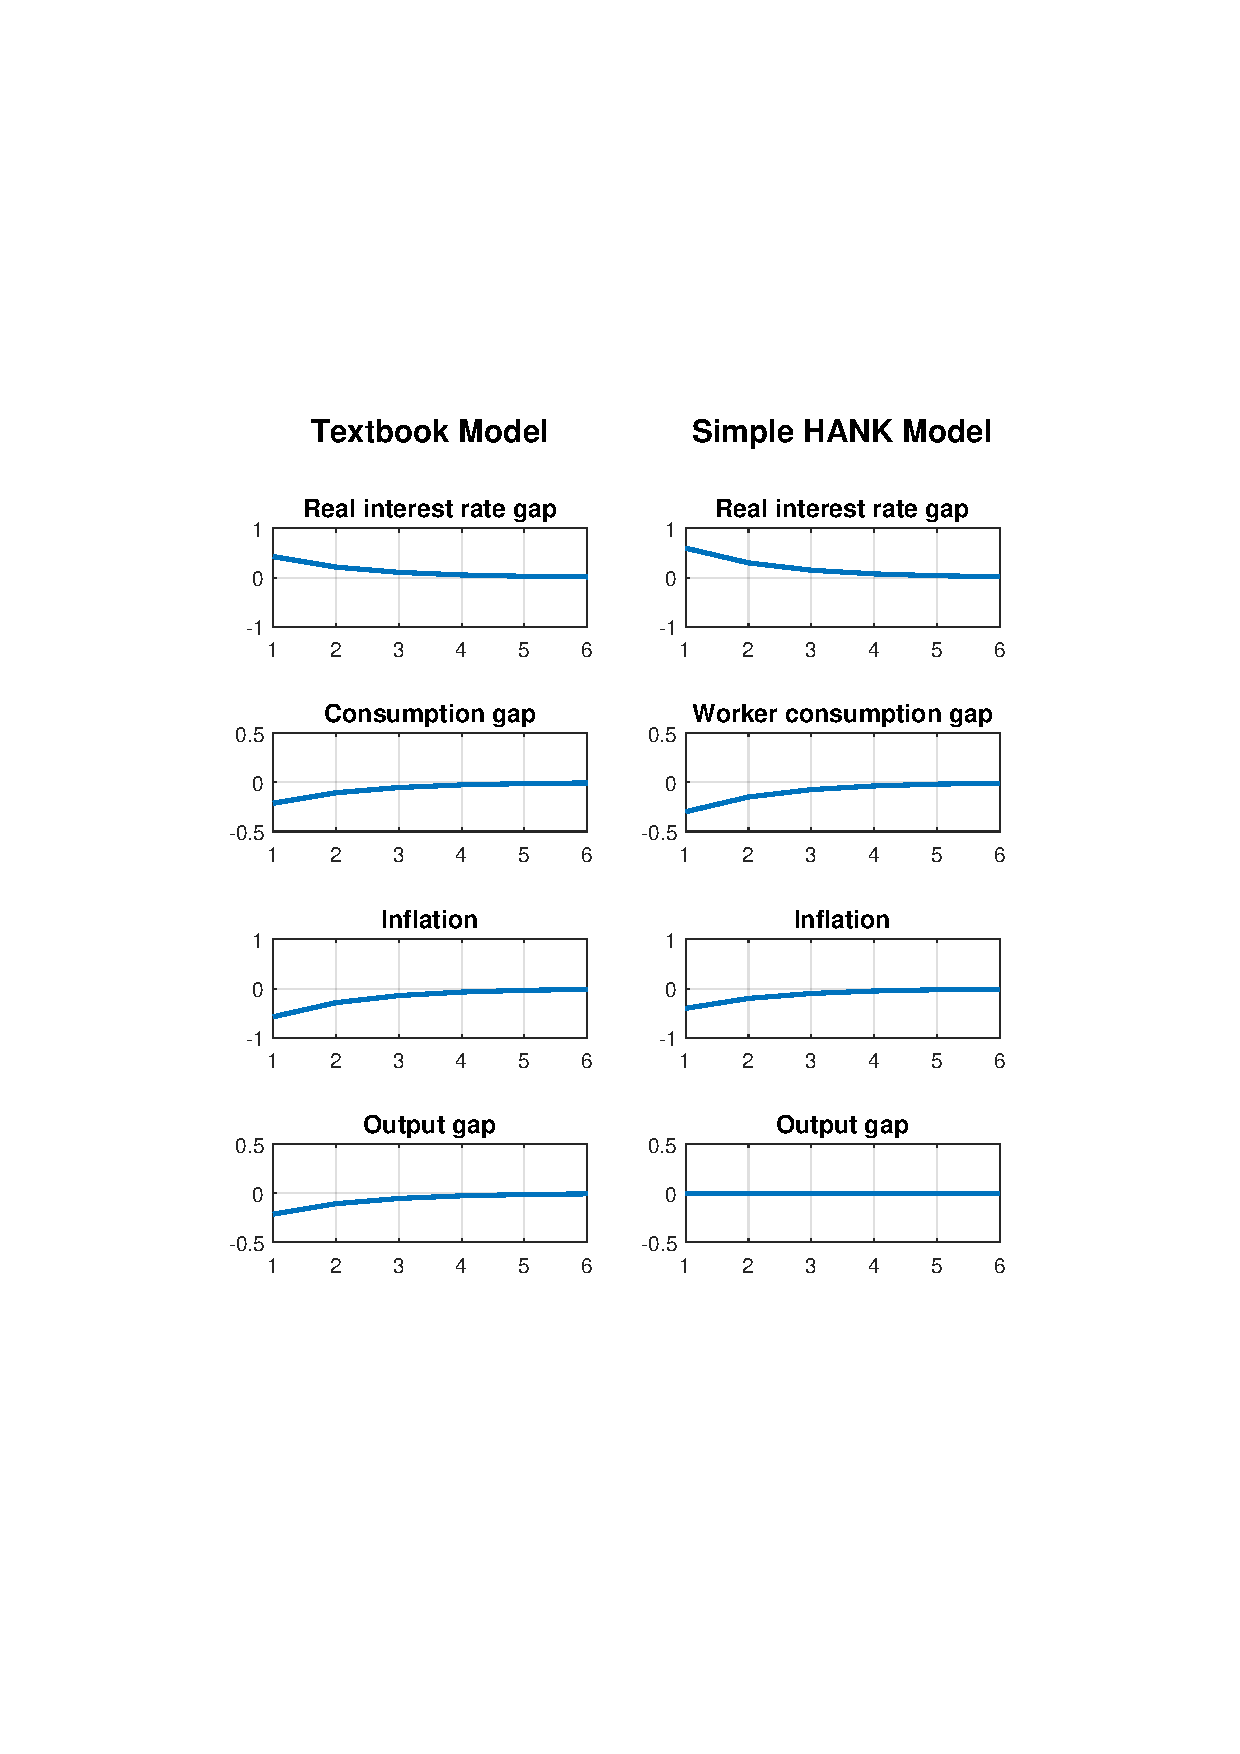
\includegraphics[scale=0.45, trim=0cm 7cm 0cm 7cm, clip]{figures/flex_wages2.pdf}
\end{flushleft}
\end{figure}
\end{frame}


\begin{frame}[t]{Monetary Shock: Labor supply, wages and profits}
\begin{figure}[h] 
\begin{flushleft}
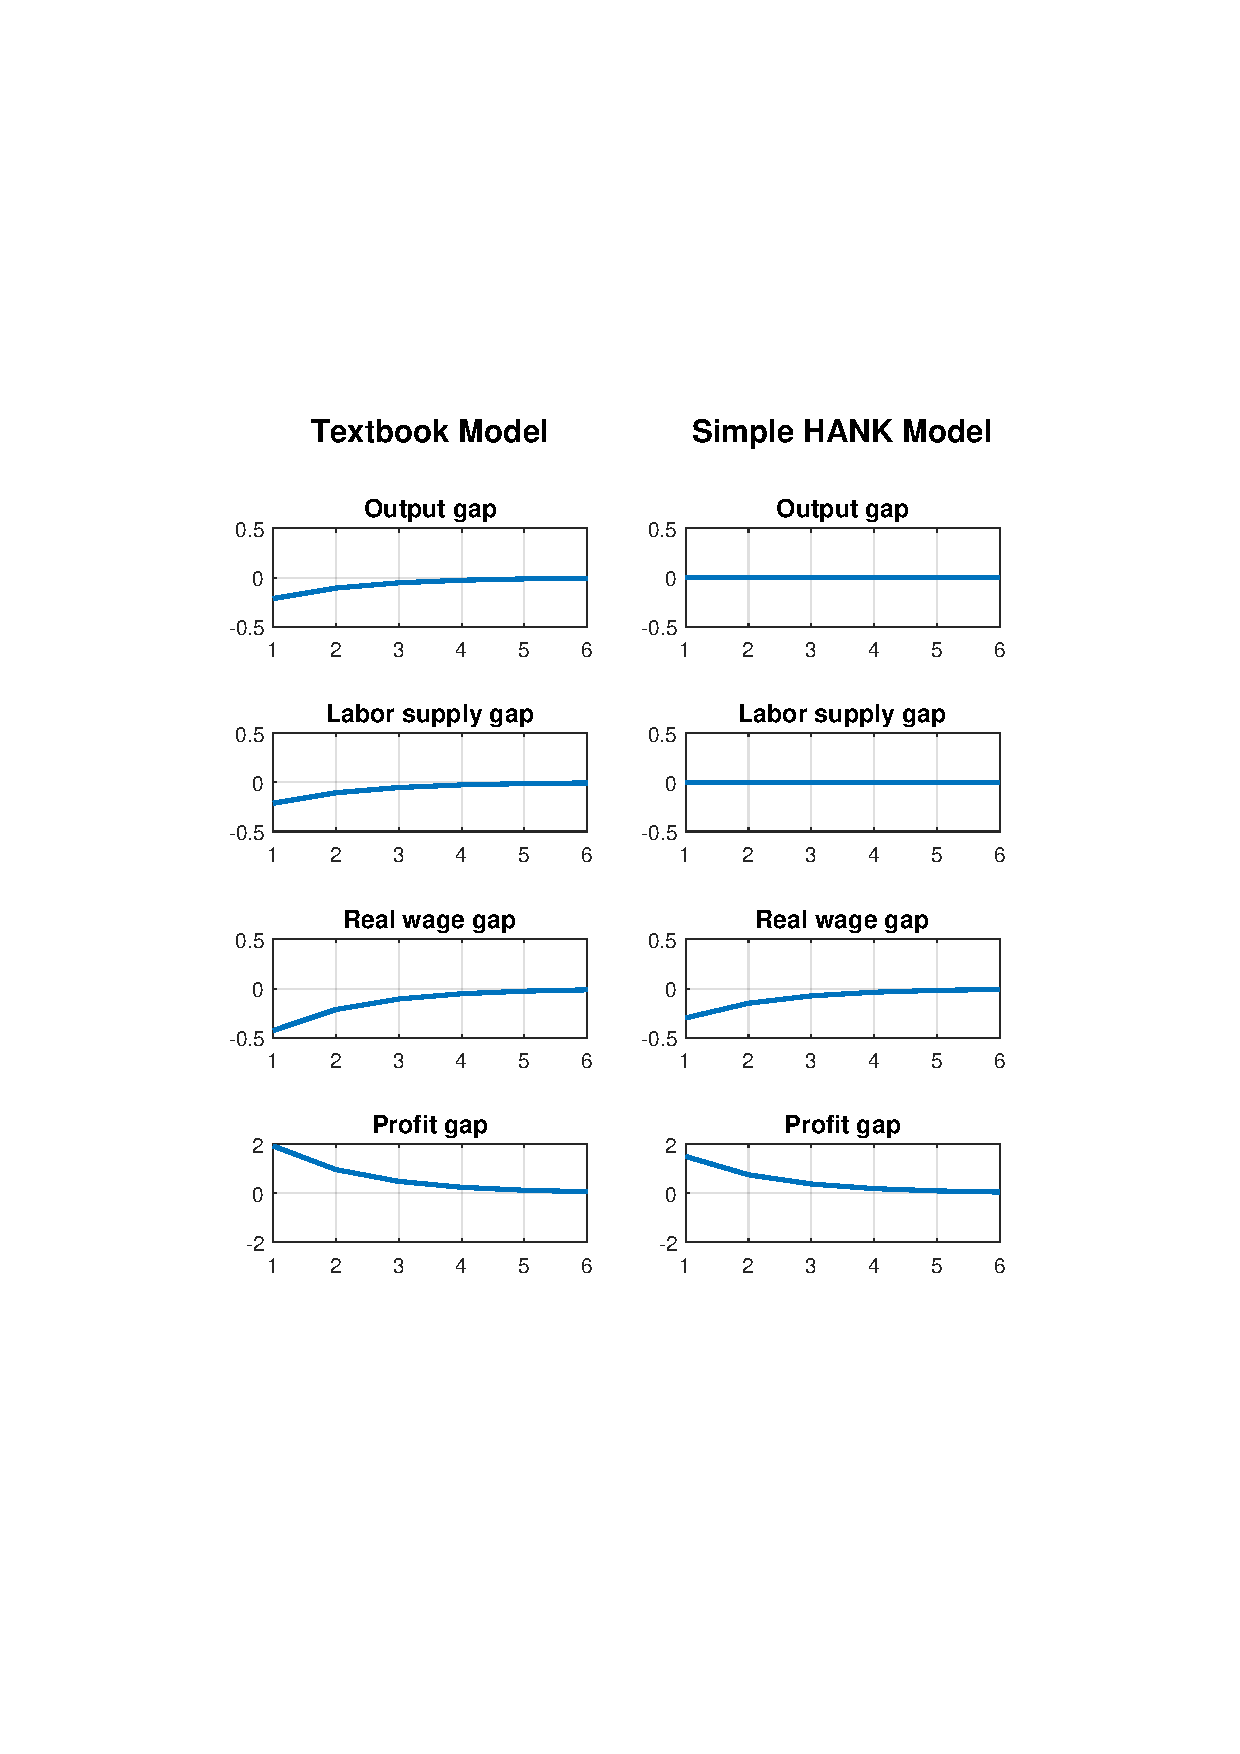
\includegraphics[scale=0.45, trim=0cm 7cm 0cm 7cm, clip]{figures/flex_wages3.pdf}
\end{flushleft}
\end{figure}
\end{frame}

\begin{frame}{The determination of labor supply}

\bit
\setlength\itemsep{1.5em}
\item Textbook RANK model -- intratemporal optimality and market clearing:
\begin{eqnarray}
&& \hat \omega_{t} = \varphi \hat n_{t} + \hat c_{t} \nonumber \\
&& \hat c_{t} = \bar{S}(\hat \omega_t  + \hat n_{t})+(1-\bar{S})\hat d_t \nonumber
\end{eqnarray}
\pause\item Equilibrium labor supply:
\begin{eqnarray}
\hat n_t = \frac{1-\bar S}{\varphi+\bar S}(\hat \omega_t-\hat d_t) \nonumber 
\end{eqnarray}
\pause\item Higher steady state profits means lower steady state labor share $\bar S$ $\rightarrow$ income effect of wages dampened
\pause\item Countercylical response in profits: direct income effect, offsetting that of procyclical wages
\eit
\end{frame}



\begin{frame}{The determination of labor supply}

\bit
\setlength\itemsep{1.5em}
\item simple HANK model -- intratemporal optimality and market clearing:
\begin{eqnarray}
&& \hat \omega_{t} = \varphi \hat n_{t} + \hat c_{t} \nonumber \\
&& \hat c_{t} = \hat \omega_t  + \hat n_{t} \nonumber
\end{eqnarray}
\pause\item Equilibrium labor supply:
\begin{eqnarray}
\hat n_t = 0 \nonumber 
\end{eqnarray}

\pause\item No profits $\rightarrow$ income and substitution effect cancel

\pause\item The zero result in the simple HANK model is due to KPR preferences, generally depends on strength of income vis-a-vis substitution effect
\eit
\end{frame}


\begin{frame}{Explanation}
\bit
\setlength\itemsep{2em}	
\item Key finding from our simple HANK model: monetary policy does not affect output

\pause 
\item Why active monetary transmission in RANK but not in HANK?

\bit
\setlength\itemsep{1em}	
\item Key difference: in RANK, working households receive profit income

\item RANK: profits respond countercyclically and dampens the relative income effect of wage fluctuations

\item HANK: income and substitution effects from wage changes cancel
\eit

\pause 
\item In other words, HANK model undoes the influence of profits on monetary transmission mechanism

%\item The difference between the HANK model and the textbook model arose in the labor supply choice

\eit
\end{frame}

\begin{frame}{Explanation}

\textbf{Take-aways}
\bit
\setlength\itemsep{1.5em}
\item What does our analysis say about the textbook RANK model?
\bit
\setlength\itemsep{0.5em}
\item Without rigid wage setting, transmission mechanism relies on
\bit
\item profits being distributed to working households
\item profits responding countercyclically
\eit
\eit
\pause

\item What does our analysis say about quantitative HANK models?
\bit
\setlength\itemsep{0.5em}
\item Heterogeneity/non-insurable income risk does not necessarily alter the equilibrium dynamics

\item The distribution of profits does alter equilibrium dynamics % when labor markets are flexible
\eit
\eit



\pause
\textbf{Does the transmission mechanism in RANK seem plausible?}

\bit 
\item No. First, very few households own firms in the real world
\item Second, most empirical evidence says that profits are procyclical: expansionary monetary policy $\rightarrow$ greater firm profits
\eit


\end{frame}


\begin{frame}{How to resolve this problem?}

\bit
\setlength\itemsep{1.5em}
\item We need a model where firm profits are procyclical, not countercyclical
\pause

\item Let's think about the form of nominal rigidities in our model
\bit
\setlength\itemsep{0.5em}
\item Rigid prices: \\ expansionary policy $\rightarrow$ wages rise faster than prices $\rightarrow$ profits fall
\item Rigid wages: \\ expansionary policy $\rightarrow$ prices rise faster than wages $\rightarrow$ profits rise
\eit

\pause
\item Next step: Introduce rigid wages to our simple HANK model, again comparing its predictions to the corresponding textbook RANK model

\eit
\end{frame}


\subsection{Introducing Rigid Wages}

\begin{frame}{Setup}

\bit

\setlength\itemsep{1em}
\item Households are differentiated by type and face CES-demand curve
\pause
\item Households can only reset their wages subject to a quadratic adjustment cost (Rotemberg, 1987)
\pause
\item Timing within period:
\ben
\item Aggregate shock is realized
\item Households choose whether to participate and set their wages
\item Idiosyncratic shocks are realized
\item Trade in goods and bond markets
\een
\pause
\item Idiosyncratic shocks are iid + $B_{jt}=0$, all HHs set the same wage 
\pause
\item $\rightarrow$ we can once more aggregate the model analytically
\pause
\item Why not Calvo friction as in Erceg-Henderson-Levin (2000)?
\bit
\item produces observationally equivalent wage Phillips curve
\item but the wage distribution depends on the aggregate state $\rightarrow$ aggregation of the Euler equation fails
\eit
\eit


\end{frame}

\begin{frame}{Production technology}

\begin{itemize}
\setlength\itemsep{1.5em}
\item Households are differentiated by type, aggregated by intermediate goods firms using CES production function
\pause
\item $\rightarrow$ Downward-sloping demand curve:
\begin{eqnarray}
N_{jt} =\frac{1}{A_{jt}} \left(\frac{\frac{W_{jt}}{A_{jt}}}{W_{t}} \right)^{-\epsilon_w} N_{t} \nonumber
\end{eqnarray}
\pause
\item and wage index:
\begin{eqnarray}
\lb{wage_index}
W_{t} &=& \left[\int_{j=0}^{1} \left(\frac{W_{jt}}{A_{jt}}\right)^{1-\epsilon_w} dj \right]^{\frac{1}{1-\epsilon_w}} \nonumber
\end{eqnarray}

\end{itemize}


\end{frame}

\begin{frame}{Worker problem}

\bit
\setlength\itemsep{1.5em}	
\item Participation utility cost $\vartheta $
\pause
\item Conditional on particpating, worker $j$ chooses $C_{jt+k}, N_{jt+k}, W_{jt+k}$ to maximize :
\begin{eqnarray}
&&  E_t \sum_{k=0}^{\infty} \beta^k \left(\log{C_{jt+k}} - \frac{N_{jt+k}^{1+\varphi}}{1+\varphi} - \vartheta\right) \nonumber \\
\text{s.t.} && P_{t+k} C_{jt+k} + Q_{t+k} B_{jt+k} = \nonumber \\
&& W_{jt+k} N_{jt+k} - \frac{\xi}{2} \left(\frac{W_{jt+k}}{W_{jt+k-1}}-1\right)^2W_{jt+k}N_{jt+k} + B_{jt+k-1} \nonumber \\
&& B_{jt+k}\geq 0  \nonumber \\
&& N_{jt} =\frac{1}{A_{jt}} \left(\frac{\frac{W_{jt}}{A_{jt}}}{W_{t}} \right)^{-\epsilon_w} N_{t} \nonumber \nonumber
\end{eqnarray}
\pause
\item As before, we set parametric conditions so that the capitalists choose not to participate.
\eit


\end{frame}

\begin{frame}{Equilibrium implications I}

\bit
\setlength\itemsep{0.5em}	
\item Becuase idiosyncratic shocks are iid and realized after wages are set, all households set the same wage $\rightarrow$ individual worker income is proportional to average worker income:
\begin{eqnarray}
W_{jt+k}N_{jt+k} = \frac{A_{jt+k}^{\epsilon_w-1}}{\left[\int_{s=0}^{1} A_{st+k}^{\epsilon_w-1} ds \right]} W_{t+k} N_{t+k} \nonumber
\end{eqnarray}
\pause

\item Since all households set the same wage, the adjustment cost is indentical to all workers 
$\rightarrow$ individual worker consumption is still proportional to average worker consumption: \pause
\begin{eqnarray}
C_{jt+k} &=& \left(1- \frac{\xi}{2} \left(\Pi^w_{t+k}-1\right)^2\right)\frac{W_{jt+k}}{P_{t+k}}N_{jt+k} \nonumber \\
&=& \left(1- \frac{\xi}{2} \left(\Pi^w_{t+k}-1\right)^2\right) \frac{A_{jt+k}^{\epsilon_w-1}}{\left[\int_{s=0}^{1} A_{st+k}^{\epsilon_w-1} ds \right]}  \frac{W_{t+k} }{P_{t+k}}N_{t+k} \nonumber \\
&=& \frac{A_{jt+k}^{\epsilon_w-1}}{\left[\int_{s=0}^{1} A_{st+k}^{\epsilon_w-1} ds \right]}  C_{t+k} \nonumber
\end{eqnarray}	





\eit


\end{frame}

\begin{frame}{Equilibrium implications II}

\bit
\setlength\itemsep{1.5em}	
\item Since all households set the same wage, and worker consumption is proportional to aggregate consumption, we retrieve a standard wage Phillips curve:
\begin{eqnarray}
\pi^w_{t} &=& \beta E_t \pi^w_{t+1} - \lambda_w(\hat \omega_t-\hat{mrs}_t) \nonumber \\
&=& \beta E_t \pi^w_{t+1} - \lambda_w(\hat \omega_t-( \hat c_t + \varphi \hat n_t)) \nonumber
\end{eqnarray}
where $\lambda_w = \frac{\epsilon_w-1}{\xi}$
\pause
\item Because idiosyncratic shocks are iid and worker consumption is proportional to aggregate consumption, the euler equation aggregates as before:
\begin{eqnarray}
\hat c_t &=& E_t \hat c_{t+1} - (\hat i_t - E_t \pi_{t+1}) \nonumber 
\end{eqnarray}
\eit


\end{frame}
\begin{frame}{Summary of log-linearized equilibrium}
\bit
\item Textbook RANK model:
\begin{eqnarray}
\lb{rep_RW_Phillips_final}
\text{Phillips}: && \pi^p_t = \beta E_t \pi^p_{t+1}+\lambda_p \hat{\omega}_t \nonumber \\
\lb{rep_RW_Phillips_wage_final}
\text{Wage Phillips}: && \pi^w_{t} = \beta E_t \pi^w_{t+1} - \lambda_w(\hat \omega_t-(\hat c_t + \varphi \hat n_t))\nonumber \\
\lb{rep_RW_wage_accounting}
\text{Wage accounting}: && \hat \omega_t = \hat \omega_{t-1} + \pi^w_t-\pi^p_t \nonumber \\
\lb{rep_RW_IS_final}
\text{IS}: && \hat c_t = E_t \hat c_{t+1} - (\hat i_t - E_t \pi_{t+1}) \nonumber \\
\lb{rep_RW_Taylor_final}
\text{Taylor rule}: && \hat i_t = \phi_{\pi}\pi^p_t + \nu_t \nonumber \\
\lb{rep_RW_MC_final}
\text{Market clearing}: && \hat c_{t} = \bar{S}(\hat \omega_t  + \hat n_{t})+(1-\bar{S})\hat d_t \nonumber
\end{eqnarray}
\eit


\bit
\item Our simple HANK model:
\begin{eqnarray}
\lb{RW_Phillips_final}
\text{Phillips}: && \pi^p_t = \beta E_t \pi^p_{t+1}+\lambda_p \hat{\omega}_t \nonumber \\
\lb{RW_Phillips_wage_final}
\text{Wage Phillips}: && \pi^w_{t} = \beta E_t \pi^w_{t+1} - \lambda_w(\hat \omega_t-(\hat c_t + \varphi \hat n_t)) \nonumber \\
\lb{RW_wage_accounting}
\text{Wage accounting}: && \hat \omega_t = \hat \omega_{t-1} + \pi^w_t-\pi^p_t \nonumber \\
\lb{RW_IS_final}
\text{IS}: && \hat c_t = E_t \hat c_{t+1} - (\hat i_t - E_t \pi_{t+1}) \nonumber \\
\lb{RW_Taylor_final}
\text{Taylor rule}: && \hat i_t = \phi_{\pi}\pi^p_t + \nu_t \nonumber \\
\lb{RW_MC_final}
\text{Market clearing}: && \hat c_{t} = \hat \omega_t  + \hat n_{t} \nonumber
\end{eqnarray}

\eit


\end{frame}


\begin{frame}{Summary of log-linearized equilibrium}

\bit
\item Textbook RANK model:
\begin{eqnarray}
\lb{rep_RW_Phillips_final}
\text{Phillips}: && \pi^p_t = \beta E_t \pi^p_{t+1}+\lambda_p \hat{\omega}_t \nonumber \\
\lb{rep_RW_Phillips_wage_final}
\text{Wage Phillips}: && \pi^w_{t} = \beta E_t \pi^w_{t+1} - \lambda_w(\hat \omega_t-(\hat c_t + \varphi \hat n_t))\nonumber \\
\lb{rep_RW_wage_accounting}
\text{Wage accounting}: && \hat \omega_t = \hat \omega_{t-1} + \pi^w_t-\pi^p_t \nonumber \\
\lb{rep_RW_IS_final}
\text{IS}: && \hat c_t = E_t \hat c_{t+1} - (\hat i_t - E_t \pi_{t+1}) \nonumber \\
\lb{rep_RW_Taylor_final}
\text{Taylor rule}: && \hat i_t = \phi_{\pi}\pi^p_t + \nu_t \nonumber \\
\lb{rep_RW_MC_final}
\text{Market clearing}: && {\color{red}\hat c_{t} = \bar{S}(\hat \omega_t  + \hat n_{t})+(1-\bar{S})\hat d_t} \nonumber
\end{eqnarray}
\eit

\bit
\item Our simple HANK model:
\begin{eqnarray}
\lb{RW_Phillips_final}
\text{Phillips}: && \pi^p_t = \beta E_t \pi^p_{t+1}+\lambda_p \hat{\omega}_t \nonumber \\
\lb{RW_Phillips_wage_final}
\text{Wage Phillips}: && \pi^w_{t} = \beta E_t \pi^w_{t+1} - \lambda_w(\hat \omega_t-(\hat c_t + \varphi \hat n_t)) \nonumber \\
\lb{RW_wage_accounting}
\text{Wage accounting}: && \hat \omega_t = \hat \omega_{t-1} + \pi^w_t-\pi^p_t \nonumber \\
\lb{RW_IS_final}
\text{IS}: && \hat c_t = E_t \hat c_{t+1} - (\hat i_t - E_t \pi_{t+1}) \nonumber \\
\lb{RW_Taylor_final}
\text{Taylor rule}: && \hat i_t = \phi_{\pi}\pi^p_t + \nu_t \nonumber \\
\lb{RW_MC_final}
\text{Market clearing}: && {\color{red} \hat c_{t} = \hat \omega_t  + \hat n_{t}}  \nonumber
\end{eqnarray}

\eit



\end{frame}

\begin{frame}{A monetary experiment}
\bit
\setlength\itemsep{1.5em}
\item Assume AR(1): $\nu_t = \rho_{\nu} \nu_{t-1}+\epsilon_{\nu t}$
\item Feed in a 25 basis point shock with $\rho_{\nu}=0.5$
\item How do the two models respond?
\item Parameterization: standard, we set $\xi$ so that the wage Phillips curve has the same slope as the wage Phillips curve derived with Calvo friction, using resetting probability from Gal\'{i} (2008)
\eit
\end{frame}


\begin{frame}[t]{Monetary Shock: Consumption, Output and Inflation}
\begin{figure}[h]  
\begin{flushleft}
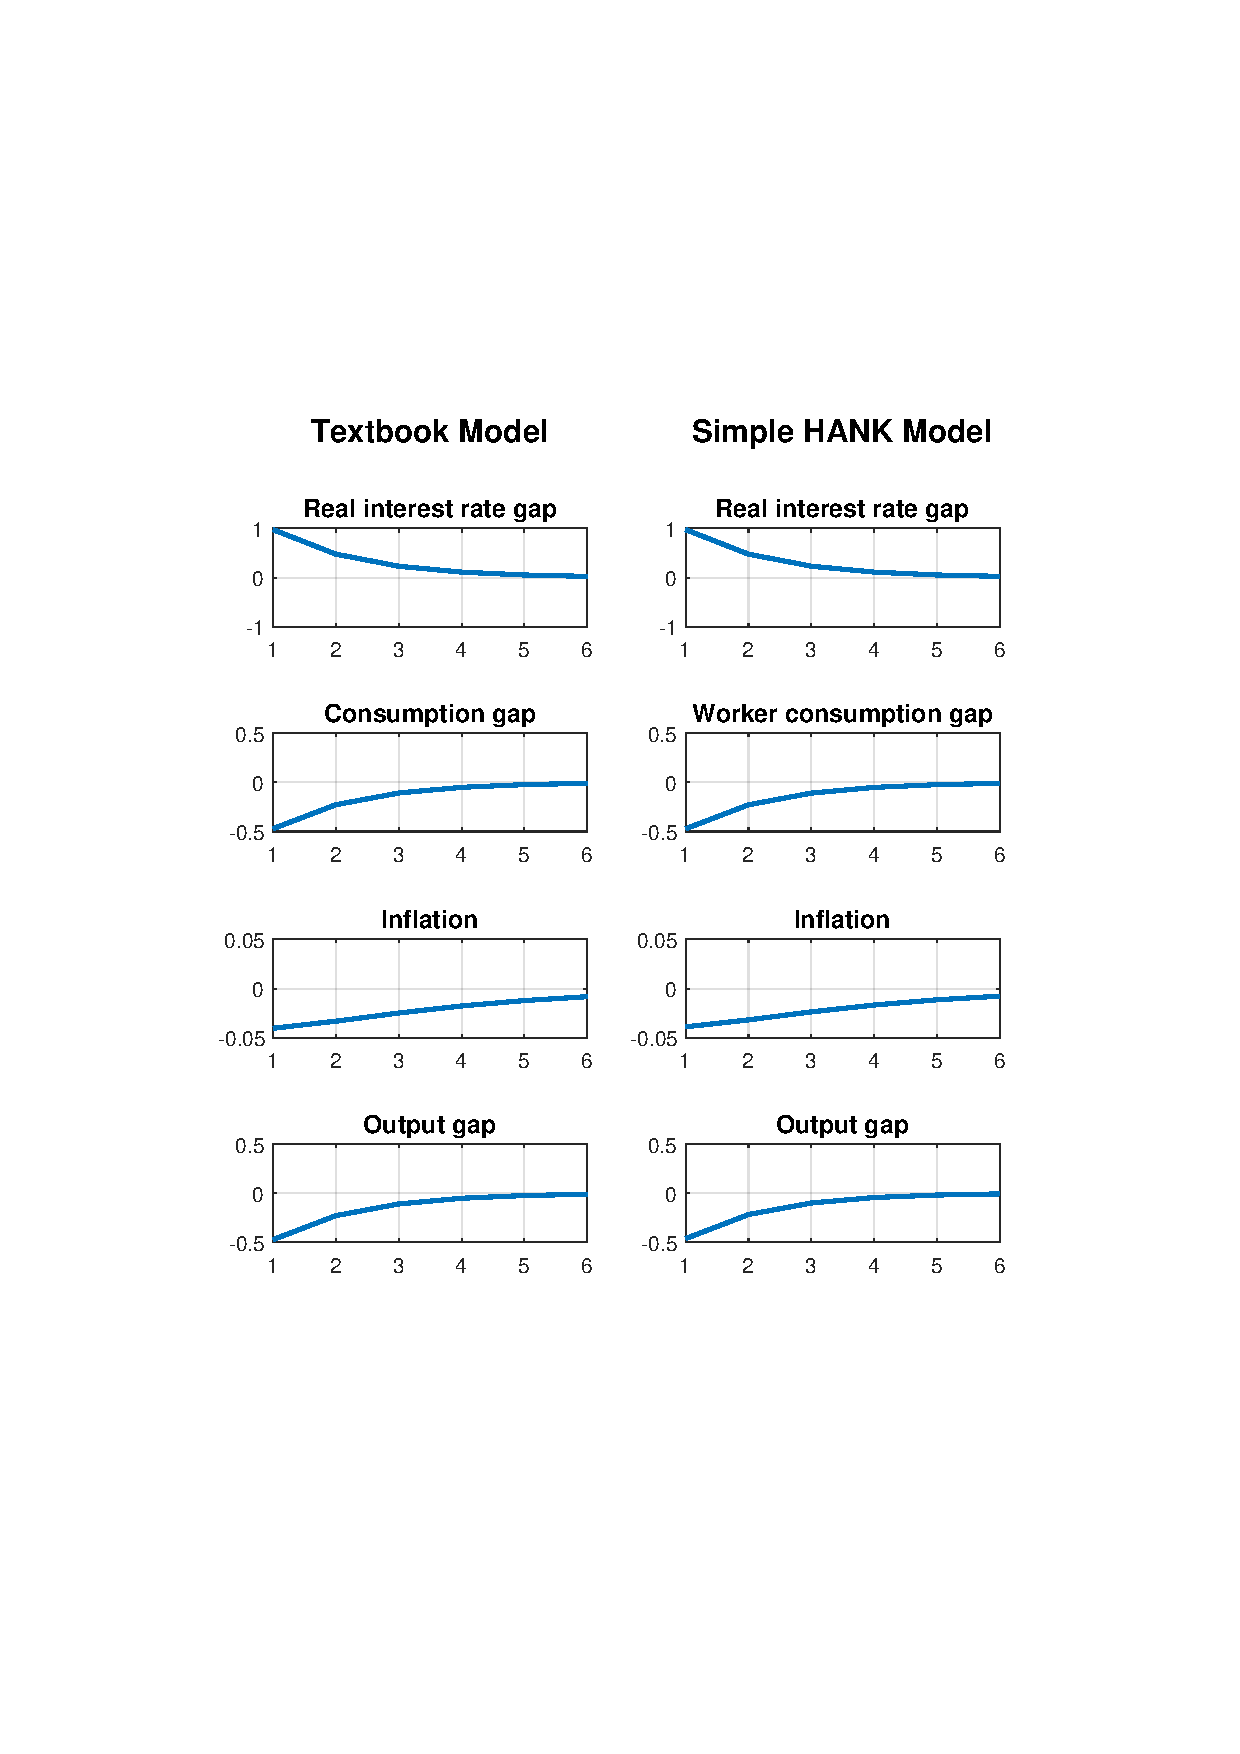
\includegraphics[scale=0.45, trim=0cm 7cm 0cm 7cm, clip]{figures/rigid_wages2.pdf}
\end{flushleft}
\end{figure}
\end{frame}


\begin{frame}[t]{Monetary Shock: Labor supply, wages and profits}
\begin{figure}[h] 
\begin{flushleft}
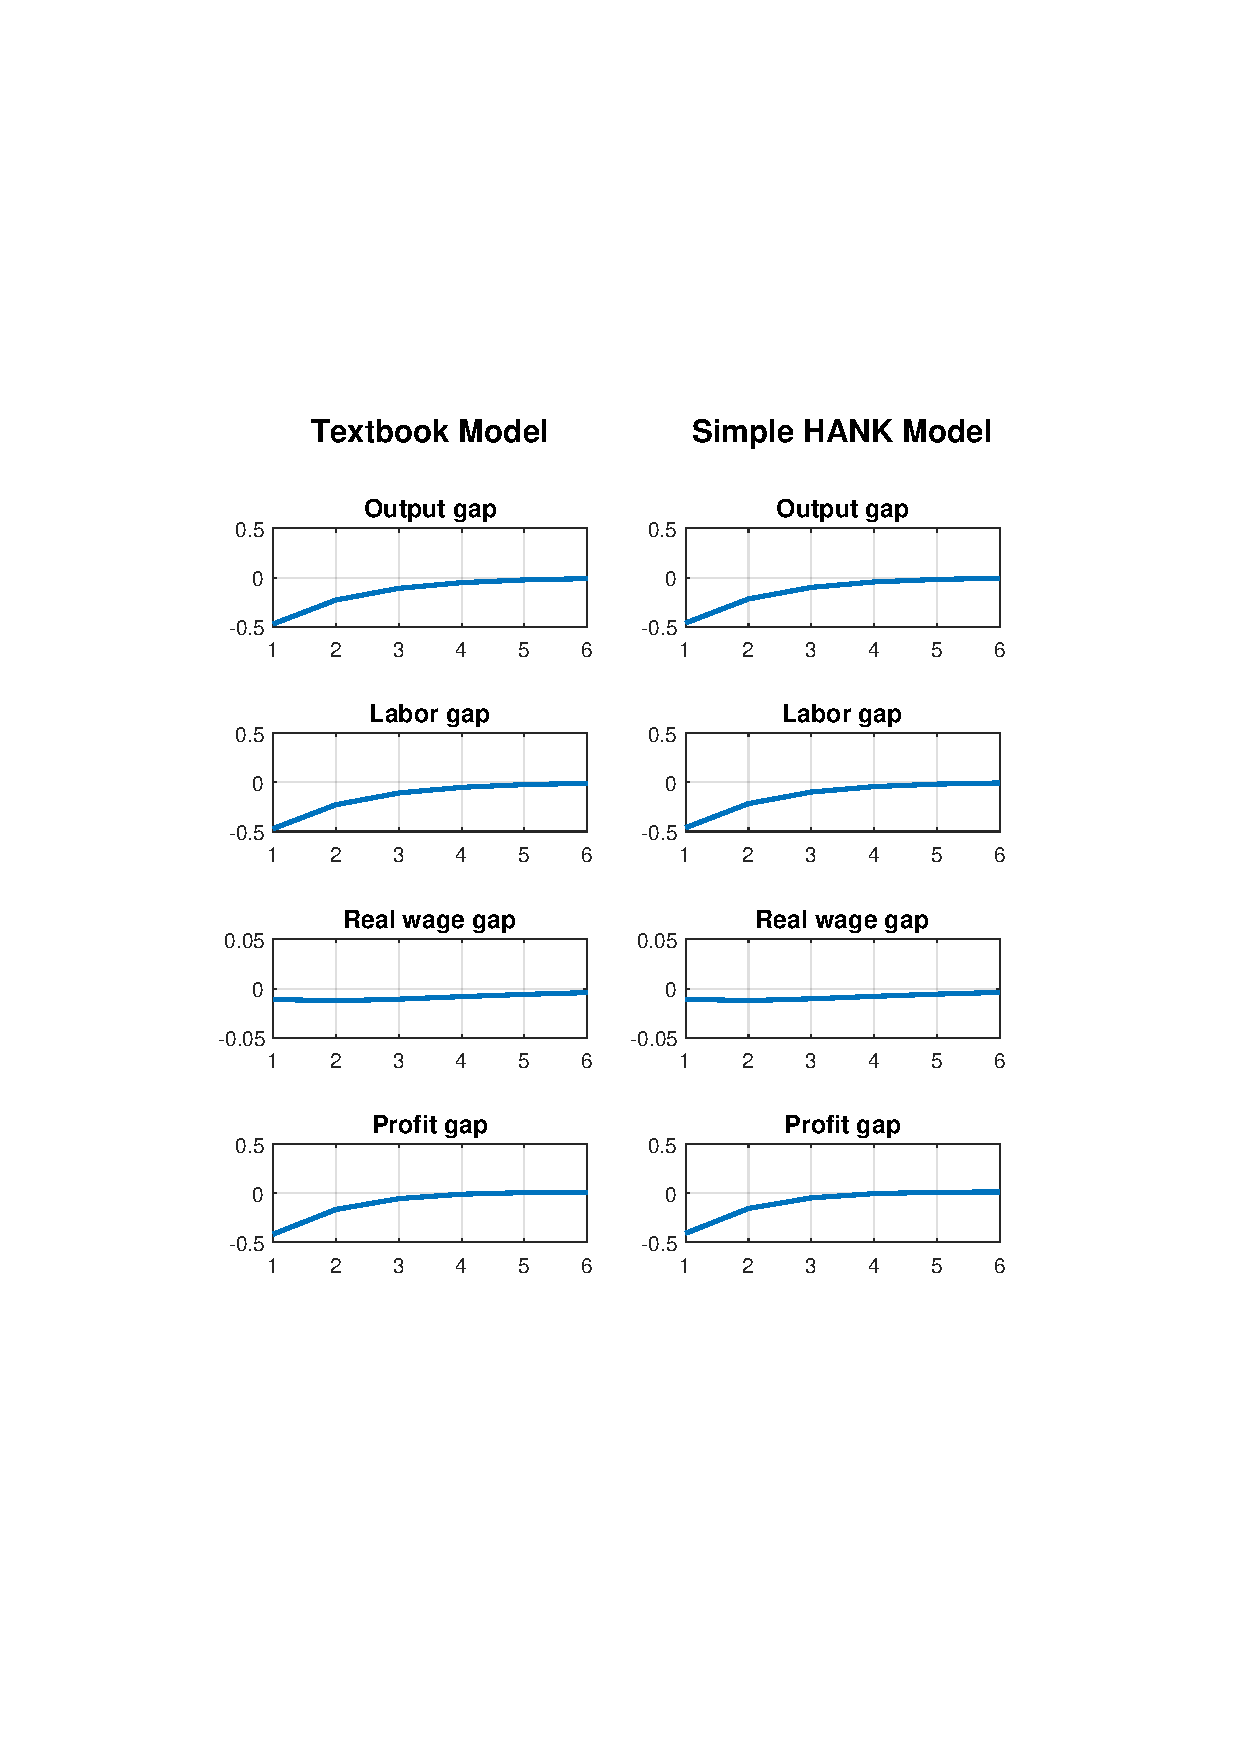
\includegraphics[scale=0.45, trim=0cm 7cm 0cm 7cm, clip]{figures/rigid_wages3.pdf}
\end{flushleft}
\end{figure}
\end{frame}

\begin{frame}{Rigid wages: Interpretation}

\bit
\setlength\itemsep{1.5em}

\item As before, real interest rate increase and worker consumption demand fall
\pause
\item With sufficiently rigid wage setting, nominal wages, inflation and real wages are all non-responsive
\pause
\item Because real wages do no respond, profits, and thus capitalist consumption demand is alinged with worker consumption
\pause
\item Goods market can only clear if labor usage respond procyclically
\pause
\item Labor usage becomes ``demand-determined''
\pause
\item No role for income and substitution effects
\eit

\end{frame}

\begin{frame}{Summary}
\ben
\setlength\itemsep{1.5em}
\item What does our analysis say about the textbook RANK model?
\bit
\setlength\itemsep{0.5em}
\item Transmission mechanism in textbook RANK model does not square well with the data
\item Monetary policy affects output because 1) profits are distributed to working households and 2) profits respond countercyclically
\eit

\pause
\item What does our analysis say about quantitative HANK models?
\bit
\setlength\itemsep{0.5em}
\item Non-insurable labor income risk does not necessarily alter the equilibrium dynamics

\item The distribution of profits does when labor markets are flexible
\eit
\pause
\item What does our analysis say about the real world? 
\setlength\itemsep{0.5em}
\bit
\item Monetary transmission mechanism only active when wages are sufficiently rigid

\item Consistent with evidence from calendar-varying VARs (Olivei-Tenreyro, 2007, 2010; Bjorklund-Carlsson-Skans, 2016)
\eit

\een
\end{frame}


%\begin{frame}[t]{Baseline model: IRF to Monetary Shock}
%\begin{figure}[h]  
%	\begin{flushleft}
%		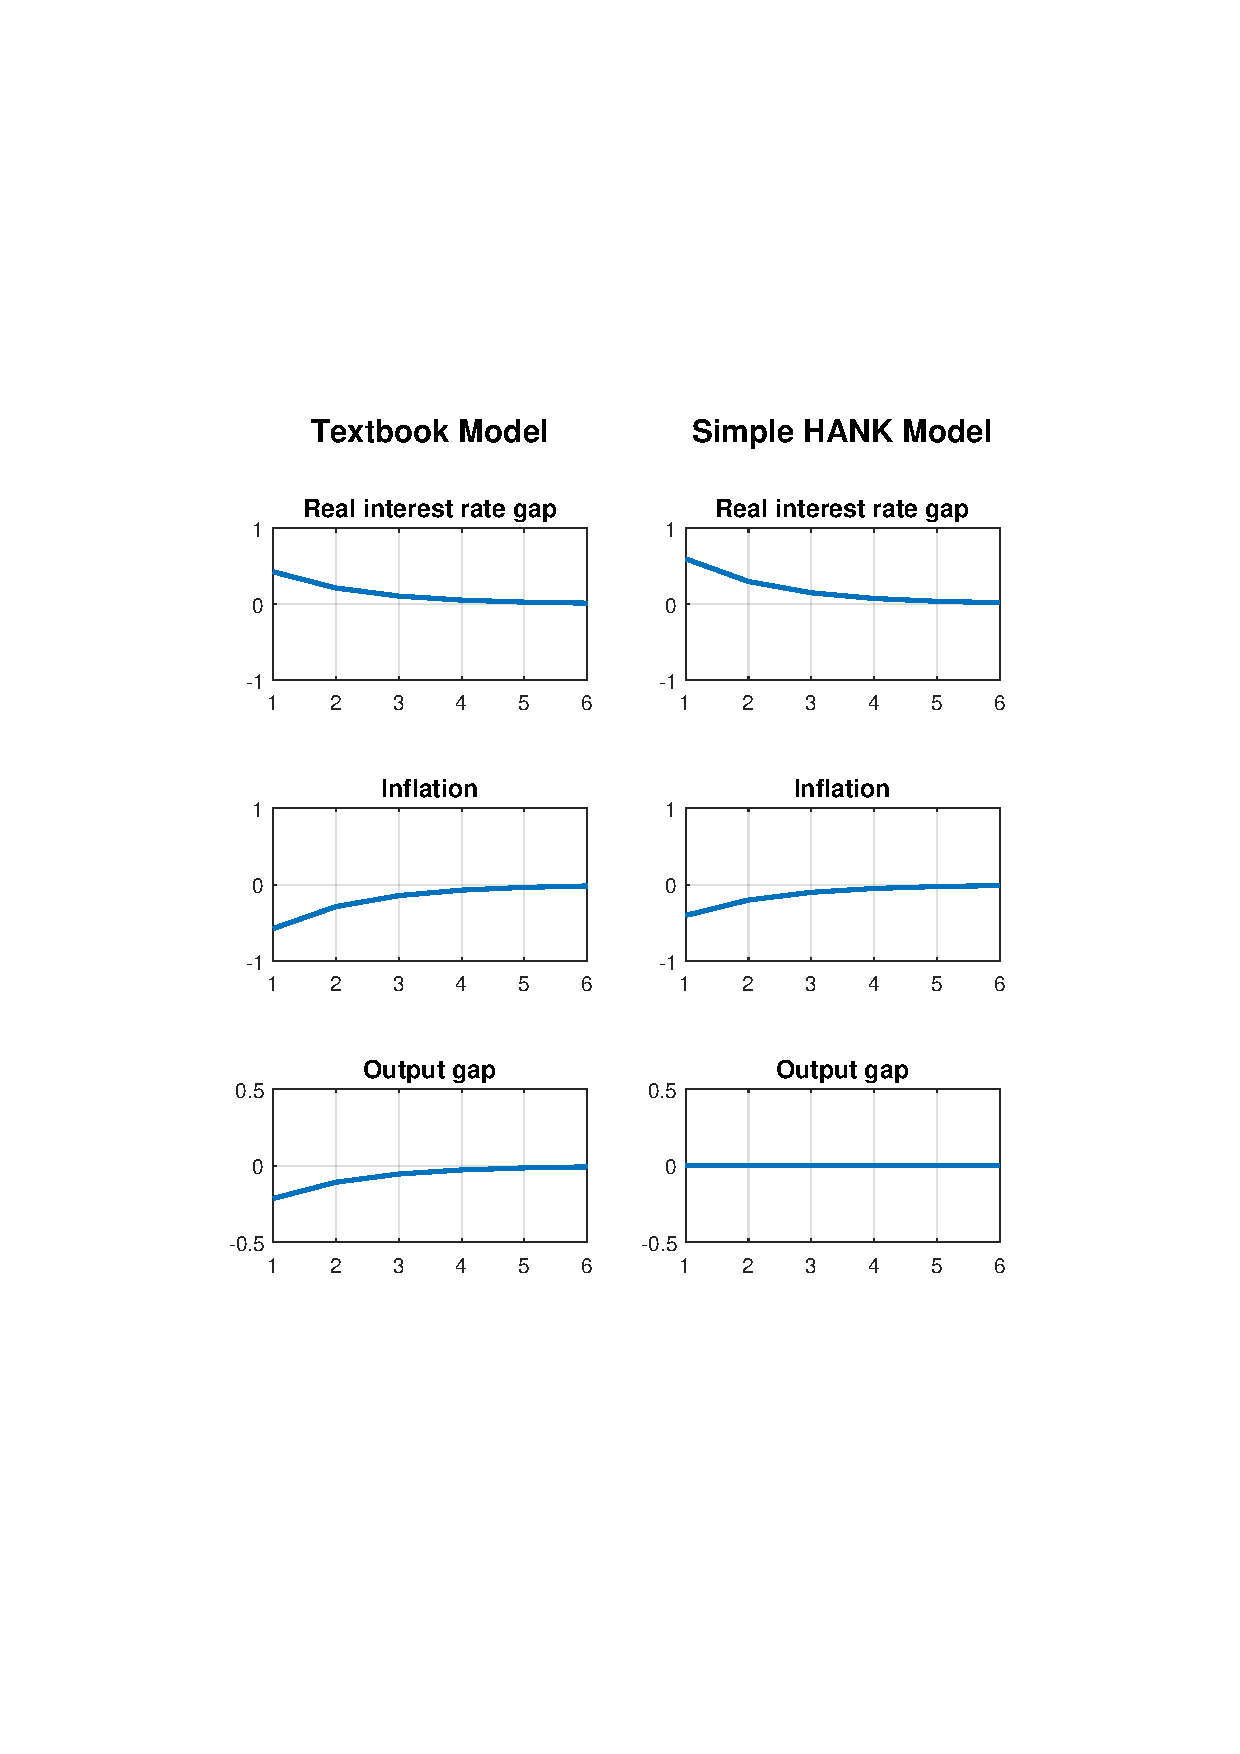
\includegraphics[scale=0.45, trim=0cm 7cm 0cm 7cm, clip]{figures/flex_wages1.pdf}
%	\end{flushleft}
%\end{figure}
%\end{frame}
%
%
%\begin{frame}[t]{Model with rigid wages: IRF to Monetary Shock}
%\begin{figure}[h] 
%\begin{flushleft}
%	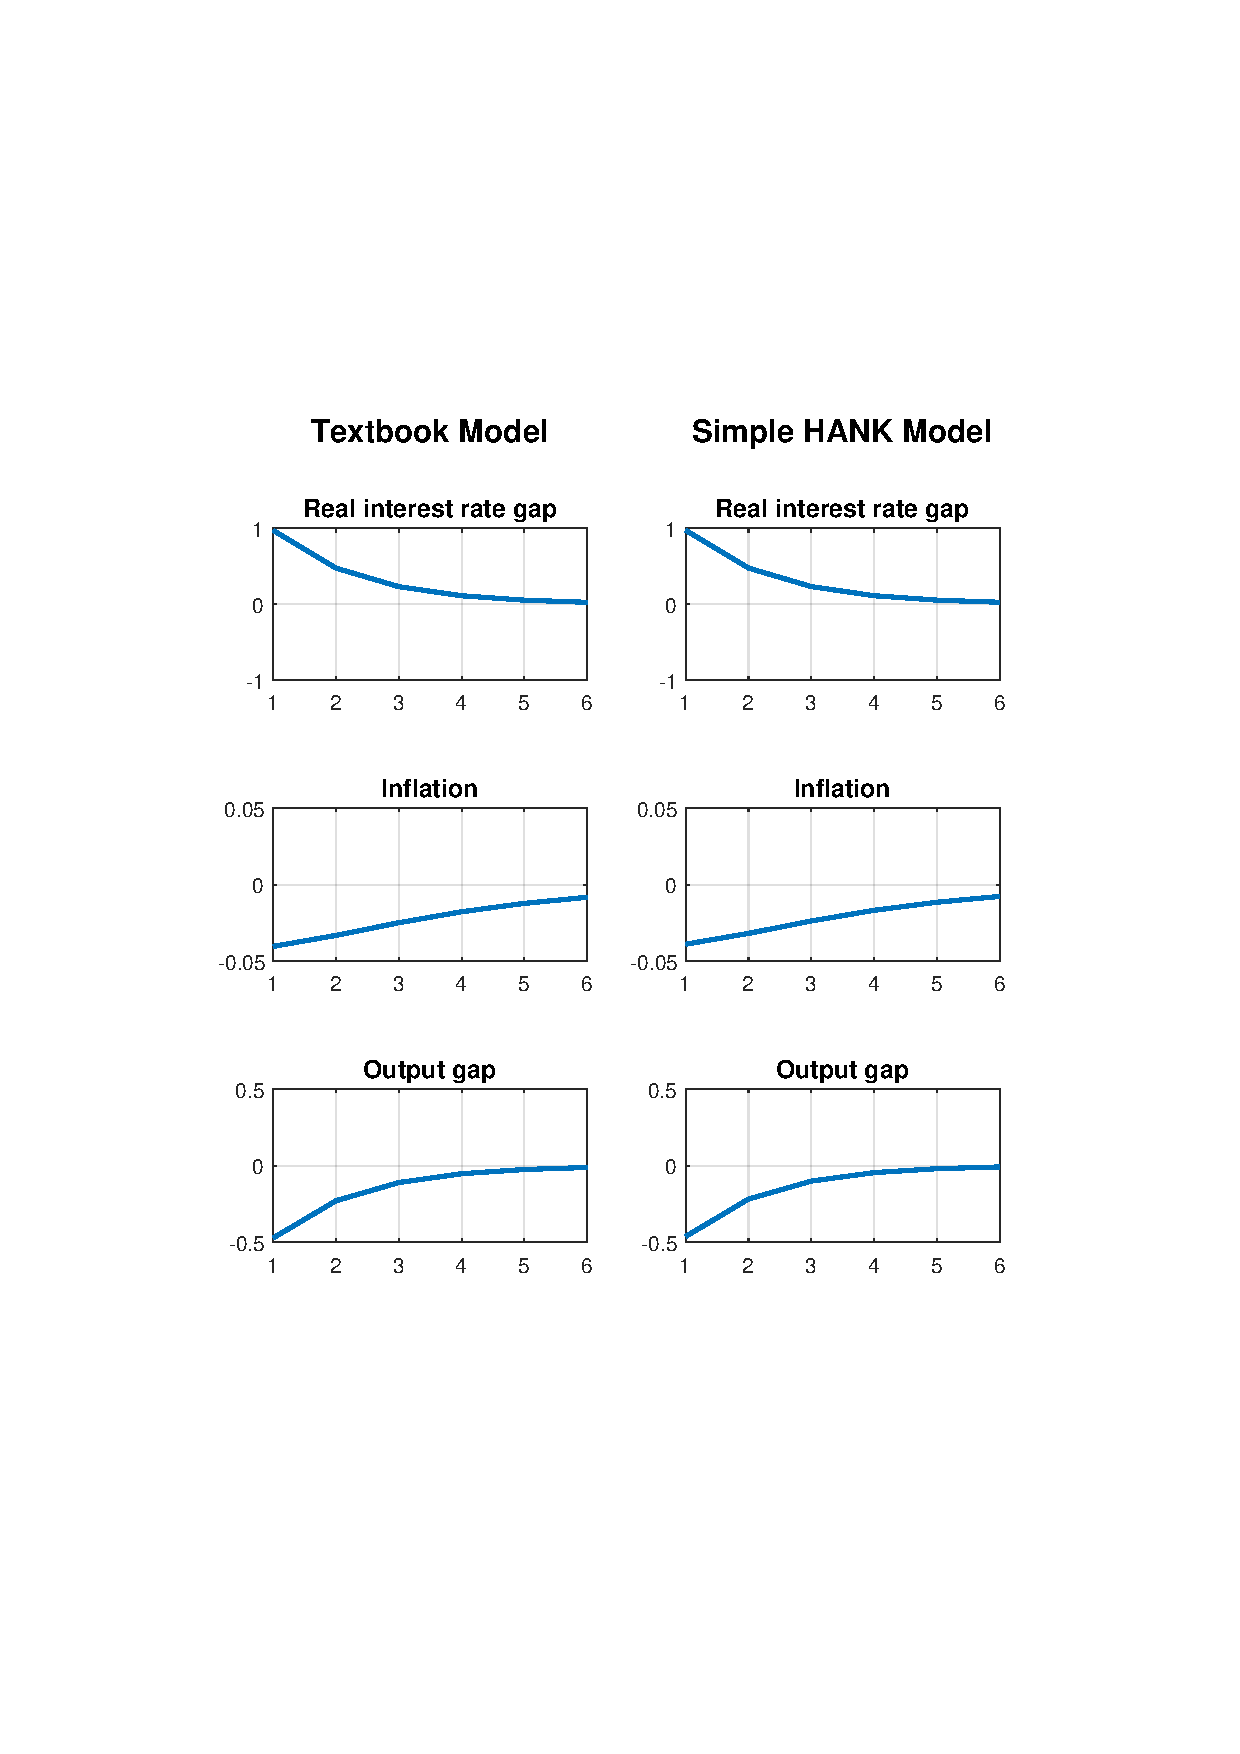
\includegraphics[scale=0.45, trim=0cm 7cm 0cm 7cm, clip]{figures/rigid_wages1.pdf}
%\end{flushleft}
%\end{figure}
%\end{frame}

\section{Fiscal Policy Transmission}


\begin{frame}{Motivation}
\bit
\setlength\itemsep{1.5em}
\item Long-standing open question: what determines the fiscal multiplier?

\begin{figure}[h]  
	\begin{flushleft}
		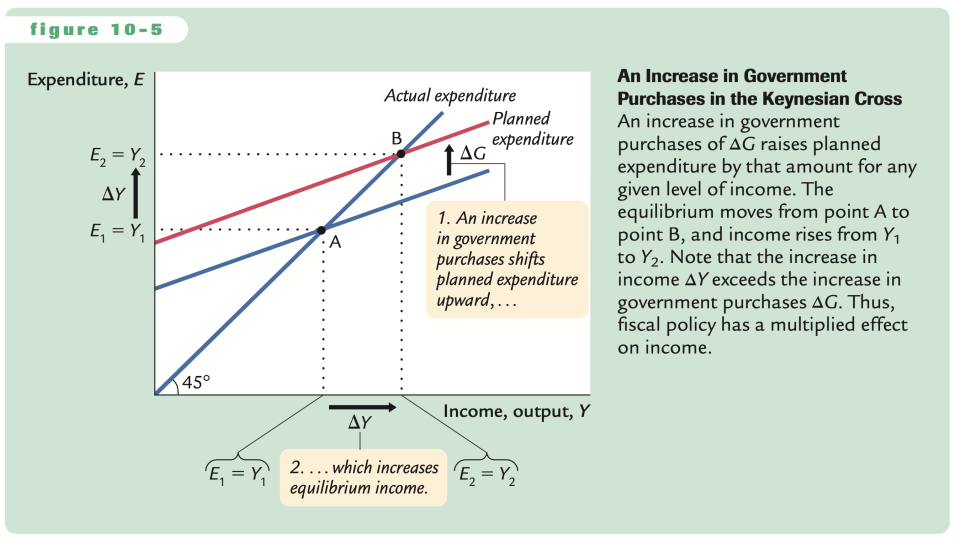
\includegraphics[scale=0.35]{figures/IKC.png}
	\end{flushleft}
\end{figure}

\pause 

\item To answer this question: will turn to Auclert, Rognlie, and Straub (2018)

\eit
\end{frame}


\section{Summary}



\begin{frame}{Summary}

\bit
\setlength\itemsep{1.5em}
\item \textbf{Previously:} Learned to solve and simulate quantitative HANK models

\pause
\item \textbf{Today:} Discussed two stylized HANK models that allow us to derive analytical insights
\bit 
\item Monetary policy: key role of profits in RANK and HANK models, important to fix the model to make the mechanism more realistic
\item Fiscal policy: derived the intertemporal Keynesian cross, showing what conditions are necessary for a fiscal multiplier greater than one
\eit 


\pause
\item \textbf{Important tool:} altering the degree of risk sharing in the economy
\bit 
\item RANK models: full risk sharing
\item Quantitative HANK models: partial risk sharing
\item Zero liquidity HANK model: no risk sharing 
\eit 

\pause
\item \textbf{Next time:} global solution methods
\eit
\end{frame}






\end{document}